% Latex template: https://github.com/mqTeXUsers/Macquarie-University-Beamer-Theme

% Slide Masters:

% Title
% Text
% 2 column
% Full-image
% Bibliography
% Closing
 
\documentclass[aspectratio=169, 11pt]{beamer} % Aspect ratio
% https://tex.stackexchange.com/a/14339/5483 
% Possible values: 1610, 169, 149, 54, 43 and 32.
% 169 = 16:9

\PassOptionsToPackage{table}{xcolor}    %https://tex.stackexchange.com/a/5365/5483

\usetheme{macquarie}
\usepackage{multicol} % https://tex.stackexchange.com/a/396018/5483
\usepackage{xurl}
\usepackage[british]{babel}       % Set language
% \usepackage[utf8x]{inputenc}      % Set encoding
\usepackage{colortbl}
\mode<presentation>           % Set options
{
  \usetheme{default}          % Set theme
  \usecolortheme{default}         % Set colors
  \usefonttheme{default}          % Set font theme
  \setbeamertemplate{caption}[numbered] % Set caption to be numbered
}

% Uncomment this to have the outline at the beginning of each section highlighted.
%\AtBeginSection[]
%{
%  \begin{frame}{Outline}
%    \tableofcontents[currentsection]
%  \end{frame}
%}

\usepackage{graphicx}         % For including figures
\usepackage{booktabs}         % For table rules
\usepackage{hyperref}         % For cross-referencing


\usepackage{enumitem} % https://tex.stackexchange.com/a/2292/5483

%https://tex.stackexchange.com/a/371844/5483
\setbeamerfont{bibliography entry author}{size=\tiny}
\setbeamerfont{bibliography entry title}{size=\tiny}
\setbeamerfont{bibliography entry location}{size=\tiny}
\setbeamerfont{bibliography entry note}{size=\tiny}
\setbeamerfont{bibliography item}{size=\tiny}

%https://tex.stackexchange.com/q/333587/5483
%Uncomment to set (e.g.) an OSF URI for this presentation, license, etc.
\setbeamertemplate{footline}{\strut~CC-BY-4.0\hfill\insertframenumber~/~\inserttotalframenumber\strut~~~}

\usepackage{comment} % for commenting out multiple lines; uses \begin{comment} ... \end{comment}

\title{Transparency, reproducibility, and synthesis} % Presentation title
\author{A/Prof Shawn A Ross, Director of Data Science and eResearch}               % Presentation author
\institute{Office of the Deputy Vice-Chancellor (Research)}         % Author affiliation
\date{Monday 18 November 2019}                 % Today's date  
\begin{document}

% Title page
% This page includes the information defined earlier including title, author/s, affiliation/s and the date
% \begin{frame}[noframenumbering]

\begin{comment}

Abstract: 



Outline:

(1) Transparency, reproducibility, scalability today
-Reproducibility crisis
-Why? cognitive biases (ways we deceive ourselves, like confirmation bias or seeing patterns where there are none), professional pressures (journals like spectacular positive findings, not so interested in negative outcomes, despite the fact that falsification is important to the advancement of knowledge), poor research design (e.g., conflating inductive and deductive research), statistical errors
-'claimed research findings may often be simply accurate measures of the prevailing bias' \cite{Alberts2015-nq}
-Worse in social sciences and humanities: Sahlins, can you tell a paradigm from a fad? 'Paradigms change in the social sciences because,
their persuasiveness really being more political than empirical, they become commonplace universals. People get tired of them. They get bored.' \cite{Sahlins1999-is}
-Ideally, research is self-correcting, but emerging argument that active steps must be taken (new discipline of metascience)
-Response: improved research design (e.g., pre-commitment to approach, method, data collection, and analysis plan before starting research); transparency: make the process part of the product (e.g., data and analytical code)
-Should be done for its own sake, but also because otherwise archaeology will be sidelined in the emerging world of open scholarship (or, 'do you want to publish in Nature')
-Status quo so poor in archaeology that we don't even know if we have a problem (although indications are that we do...).
-Archaeology as a small data discipline has serious (but not unique) challenges.
-Problems will get worse, not better, if big data approaches like photogrametry, remote sensing, etc., come into common use without the basics (good / explicit design, FAIR data, analytical reproducibility) in place. 
-Archaeology tends to favour 'sharks and lasers'.
-Archaeology tends to neglect what is happening in neighbouring disciplines - striking difference going to the CAAs and going to RDA / CODATA - and it's the latter that feed into (e.g.) funder, publisher, and government policy
-Many of the same approaches that provide for transparency and reproducibility also contribute to scalability of research. Scalability arises largely from the ability to combine evidence ('data') from many sources, which requires that the data be technically and semantically interoperable. Such data is encouraged by FAIR principles and use of domain repositories (for example), automate routine processes (e.g., using the same code-based approaches that support analytical reproducibility), but good documentation of the project (explicit and sound research design) is also necessary. 
-None of these ideas are new in archaeology, many were raised in surprisingly contemporary language by early Processualists in the 1970s \cite{Hole1973-cy} - research design should drive your fieldwork, not methods, your approach should be explicitly stated, prioritise making your data compatible with that from other projects even at the expense of missed opportunities for marginal improvement.
-In this regard, our salvation lies in a 'back to basics' processualism, not naive empiricism or post-processual high theory.


(2) What does the future look like?
-Archaeology as a data science discipline more than a fieldwork discipline
-Archaeology as a discipline where registration of research design is routine (and all projects have a design: inductive / deductive / idiographic / nomothetic...research questions or hypotheses).
-Data structures, field processes, methods, etc. are fully documented and published
-Comprehensive, FAIR datasets are produced and deposited in domain repositories
-Analysis shifts from Excel and ARCGIS to code
-Processes / methods, data, and code are routinely reused
-We can have reasonable confidence in our results, self-correction can happen when we are wrong, and evidence / analysis can be combined from many projects to answer big questions.


\end{comment}


\maketitle

  
% \end{frame}

% Outline
% This page includes the outline (Table of content) of the presentation. All sections and subsections will appear in the outline by default.
\begin{frame}{The context of Research Data Management}
  \tableofcontents
\end{frame}

% The following is the most frequently used slide types in beamer
% The slide structure is as follows:
%
%\begin{frame}{<slide-title>}
% <content>
%\end{frame}


% Presentation providing context for the new data governance policies and procedures at Macquarie University

\section{The reproducibility crisis}

\begin{frame}{The `reproducibility crisis'}
  For nearly a decade the reproducibility crisis has featured in the scientific literature \cite{Jasny2011-bw, Baker2016-cf, Munafo2017-bj}. Low reproducibility rates have emerged from large-scale studies:
    \begin{itemize}[label=\textbullet]
        \item Results from only 39\% of psychology studies could be reproduced \cite{Open_Science_Collaboration2015-vf}.
        \item Even lower reproducibility rate in biomedical research \cite{Begley2012-xt,Prinz2011-za}.
    \end{itemize}
\end{frame}

\begin{frame}{Perceptions of the reproducibility crisis}
  \begin{figure}[H]
    \centering
        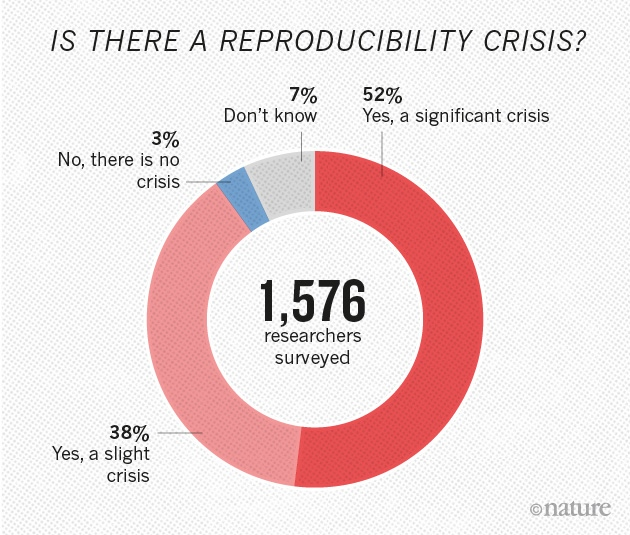
\includegraphics[height=.7\textheight]{figures/reproducibility-graphic-online1.jpeg}
        \caption{Is there a reproducibility crisis? \cite{Baker2016-cf}}
        \label{fig:Baker2016}
  \end{figure}
\end{frame}

\section{Causes of the crisis}

\begin{frame}{Data loss}
 \begin{figure}[H]
    \centering
        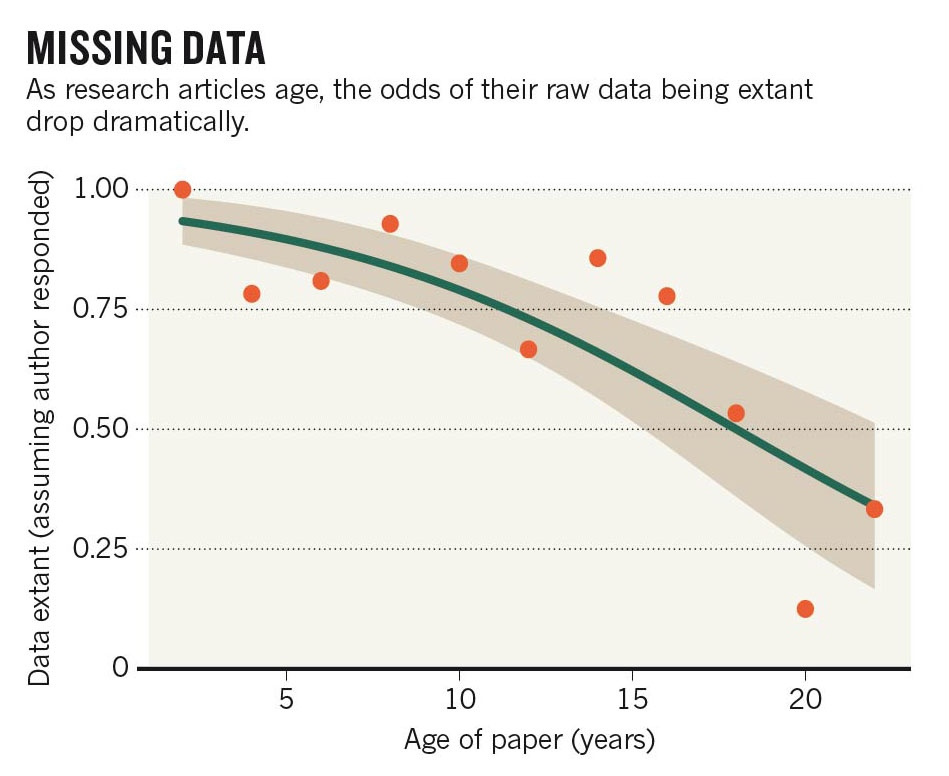
\includegraphics[height=.75\textheight]{figures/Missing-Data.png}
        \caption{\cite{Vines2014-zr}}
        \label{fig:vines2014}
 \end{figure}
\end{frame}

\begin{frame}{Other causes}
    \begin{itemize}[label=\textbullet]
        \item Destructive editing of data and irreproduciple analysis.
        \item Professional pressures.
        \item Cognitive biases.
    \end{itemize}
    `Claimed research findings may often be simply accurate measures of the prevailing bias'. \cite{Alberts2015-nq} \par
\end{frame}

\section{Responses to the crisis}

\begin{frame}{Self-correction}
Ideally, research is self-correcting, but active steps must be taken.
    \begin{itemize}[label=\textbullet]
        \item Improved research design (e.g., pre-commitment to approach, method, data collection, and analysis plan before starting research).
        \item Transparency around evidence and analysis (e.g., provide comprehensive datasets and analytical code).
    \end{itemize}
\end{frame}

\begin{frame}{Better data and analytical practice}
  Manifestos, statements, and guidelines:
    \begin{itemize}[label=\textbullet]
        \item OECD Priniples and Guidelines for Access to Research Data \cite{Oecd2007-vi}.
        \item Findable, Accessible, Interoperable, and Reusable (FAIR) data \cite{Wilkinson2016-mr, Go-fair2017-vs}.
        \item Transparency and Openness Promotion (TOP) guidelines \cite{Nosek2015-wm, Cos2019-mr}.
        \item Data transparency toolkit \cite{Perkel2018-rw}.
    \end{itemize}
\end{frame}

\begin{frame}{Archaeology in this context}
    \begin{itemize}[label=\textbullet]
        \item We do not even know how bad the problem is.
        \item Archaeology as a `small data' discipline has serious (but not unique) challenges that are rarely recognised.
        \item In technology, some preference for `sharks with lasers' over difficult and painstaking data management. 
        \item Problems will get worse, not better, if bigger data approaches like photogrammetry, remote sensing, etc., come into common use without the fundamentals of data practice in place.
        \item Archaeology tends to be somewhat provincial - striking difference between level of discourse at Computer Applications in Archaeology conferences versus, say, Research Data Alliance or CODATA. 
    \end{itemize}
\end{frame}

\begin{frame}{Journal transparency mandates}
  Good practice should be done for its own sake, but also to avoid being sidelined as a discipline in the emerging world of Open Scholarship. \par
  Example mandates for transparency or reproducibility:
    \begin{itemize}[label=\textbullet]
        \item Nature: Transparency Upgrade \cite{Nature2017-lq}.
        \item Nature: FAIR data in Earth science \cite{Nature2019-ng}.
        \item Copernicus: FAIR data in atmospheric sciences \cite{Van_Edig2018-bu}.
        \item TOP Guidelines signatories include publishers representing 1000+ journals, as well as professional organisations and major private foundations  \cite{Cos2019-mr}.
    \end{itemize}
\end{frame}

% https://tex.stackexchange.com/a/2292/5483
% https://ctan.org/pkg/enumitem?lang=en

\begin{frame}{Level 2 TOP Guidelines for authors (excerpt)}
  
    \begin{enumerate}[label=\arabic*.]
        \setcounter{enumi}{1}
        % This increments the enumerate counter by 1.
        
        \item Authors using original data must:
        \begin{enumerate}[label=\alph*.]
            \item make the data available at a trusted digital repository [...]
            \item include all variables, treatment conditions, and observations described in the manuscript.
            \item provide a full account of the procedures used to collect, preprocess, clean, or generate the data.
            \item provide program code, scripts, codebooks, and other documentation sufficient to precisely reproduce all published results.
            \item provide research materials and description of procedures necessary to conduct an independent replication of the research.
        \end{enumerate}
    \end{enumerate}
    \cite{Osf2014-pf}
\end{frame}

\begin{frame}{TOP Guidelines: publisher adoption}
  \begin{figure}[H]
    \centering
        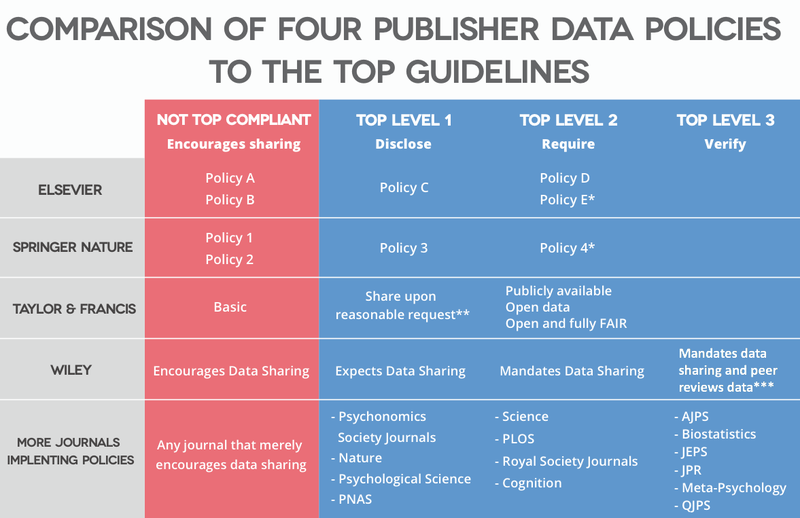
\includegraphics[height=.7\textheight]{figures/TOP-landscape.png}
        \caption{The Landscape of Open Data Policies \cite{Mellor2018-bf}}
        \label{fig:figure2}
  \end{figure}
\end{frame}

\begin{frame}{TOP Guidelines: funder endorsement}
  Private funders have endorsed via the Open Funders Research Group:
    \begin{itemize}[label=\textbullet]
        \item Alfred P. Sloan Foundation
        \item American Heart Association
        \item Bill and Melinda Gates Foundation
        \item Howard Hughes medical Institute
        \item John Templeton Foundation
        \item Laura and John Arnold Foundation
        \item Open Society Foundations
        \item Robert Wood Johnson Foundation
        \item Wellcome Trust
        \item and six more \cite{Ofrg2019-pq}
    \end{itemize}
\end{frame}

\begin{frame}{Other Funder data policies}
  \begin{figure}[H]
    \centering
        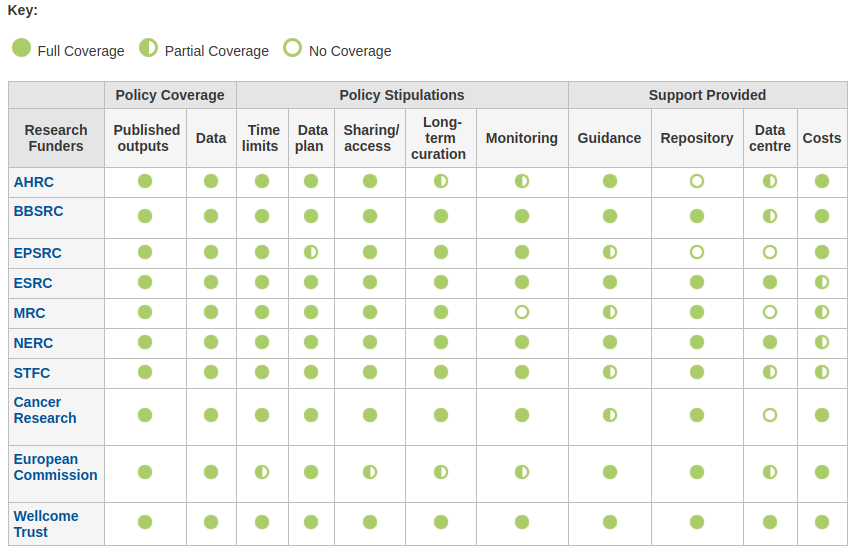
\includegraphics[height=.7\textheight]{figures/DCC-Funders.png}
        \caption{Overview of funders' data policies \cite{Dcc2019-jn}}
        \label{fig:Dcc2018}
  \end{figure}
\end{frame}

\begin{frame}{EU research governance policy}
  With the Horizon 2020 program \cite{European_Commission2019-an} Europe made 'research data open by default':
    \begin{itemize}[label=\textbullet]
        \item `Participating projects will be required to develop a \textbf{Data Management Plan} (DMP), in which they will specify \textbf{what data will be open}: detailing \textbf{what data the project will generate}, whether and how it will be \textbf{exploited or made accessible for verification and re-use}, and how it will be \textbf{curated and preserved}.'
        \item Opt-outs: 'as open as possible, as closed as necessary'.
        \item Associated costs can be claimed in grant.
        \item Continuing investment, e.g., FAIRsFAIR project \cite{Knaw-dans2019-sv} to implement FAIR across repositories.
    \end{itemize}
\end{frame}

\begin{frame}{Not just the natural sciences}
  Changes are coming to HASS disciplines:
    \begin{itemize}[label=\textbullet]
        \item American Journal of Political Science requires (and tests) data and code \cite{Jacoby2017-lw, Ajps2015-ex}.
        \item All European Academies (allea) E-Humanities working group \cite{Allea2019-wy} has issued an Open Consultation on `Sustainable and FAIR Data Sharing in the Humanities' \cite{Allea2019-aw}.
        \item Allea seeks to address the imperatives of the `Open Science agenda' across Humanities and Social Sciences, and `facilitate the adoption of Open Science across the Humanities'.
        \item Research Data Alliance (RDA) has an 'Ambassador for the Humanities' and is examining how RDA standards and outputs can apply to humanities disciplines \cite{Rda2019-wc}.
    \end{itemize}
\end{frame}

\begin{frame}{Challenges in HASS disciplines}
  In the current environment, we need to demonstrate how robust and reliable our research is. Considering the evidence we use, however, HASS faces legal and technical challenges to showing our work:
    \begin{itemize}[label=\textbullet]
        \item Copyright: texts, archival documents, films and audio recordings, secondary sources.
        \item For evidence that is online, links and references possible (but access may have a cost); if not online, the tyranny of distance re-asserts itself (if access is possible at all). 
        \item Technical: 'small data' problems, including diverse and heterogenous data of various types, plus data and methods often emergent from research; harder than 'big data' in many ways, requires flexible and extensible infrastructure from a poorly coordinated and poorly funded domain \cite{Borgman2015-rh}.
        \cite{Rda2019-wc}.
    \end{itemize}
\end{frame}

\begin{comment}

\begin{frame}{Australia: Data sharing in the NHMRC Statement}
    The NHMRC `strongly encourages' data sharing in the National Statement on Ethical Conduct in Human Research and their Open Access Policy. \cite{Nhmrc2018-sj, Nhmrc2018-vn} \par
    National Statement 3.1.50 \par
    In the absence of justifiable ethical reasons (such as respect for cultural ownership or unmanageable risks to the privacy of research participants) and to promote access to the benefits of research, researchers should collect and store data or information generated by research projects in such a way that they can be used in future research projects. Where a researcher believes there are valid reasons for not making data or information accessible, this must be justified.
\end{frame}

\begin{frame}{NHMRC Open Access Policy 2018 changes}
    Key changes to the Open Access Policy (15 January 2018) \par
    Research data and metadata (2.2) \par
    NHMRC now strongly encourages researchers to take reasonable steps to share research data and associated metadata arising from NHMRC supported research.\par
    FAIR principles (2.7) \par
    Reference to the Australian F.A.I.R. principles (Findable, Accessible, Interoperable, Reusable) when publishing research literature and sharing data has been made.
\end{frame}

\begin{frame}{NHMRC Open Access Policy data sharing}
    Medatdata (4.1) \par
    The metadata for the peer-reviewed publication must be made openly accessible via an institutional repository as soon as possible but no later than 3 months from the date of publication. \par
    Data (4.2) \par
    NHMRC acknowledges the importance of making research data publicly accessible and therefore strongly encourages researchers to consider the reuse value of their data and to take reasonable steps to share research data and associated metadata arising from NHMRC supported research.
\end{frame}

\begin{frame}{Legal compliance}
    \begin{itemize}[label=\textbullet]
        \item NSW General Retention and Disposal Authority GDA 23; data associated with `significant' research or researchers must be kept forever (23.6.1) \cite{Nsw2015-kv}
        \item NSW Privacy and Personal Information Protection Act 1998 No 133, esp. Part 2, Division 1, Section 19, which flags indicators of high sensitivity and establishes data sovereignty.\cite{Nsw1998-mw} Compare the (Australian) Privacy Act 1988, esp. Part II, Division 1, Section 6 `Sensitive Information' and Schedule 1, and `Australian Privacy Principles', Section 8, which covers some university-controlled entities. \cite{Ag2017-oz,Oaic2019-ng}
        \item NSW Notifiable Data Breach guidance \cite{Ipc_nsw2018-yr}; see also the Australian Notifiable Data Breaches scheme \cite{Oaic2019-dq}
        \item EU General Data Protection Regulation \cite{Gdpr2019-ee}
    \end{itemize}
\end{frame}

\end{comment}

\section{Beyond compliance}

\begin{frame}{Large-scale research}
    The same approaches that facilitate transparency and reproducibility support the kind of scalable and synthetic research that can address archaeological `grand challenges'. \cite{Kintigh2014-ub}
        \begin{itemize}[label=\textbullet]
            \item Paper data capture and manual digitisation and cleaning don't scale.
            \item Collaboration based on email and desktop software doesn't scale.
    \end{itemize}
\end{frame}

\begin{frame}{Scalable approaches to data and analysis}
  \begin{figure}[H]
    \centering
        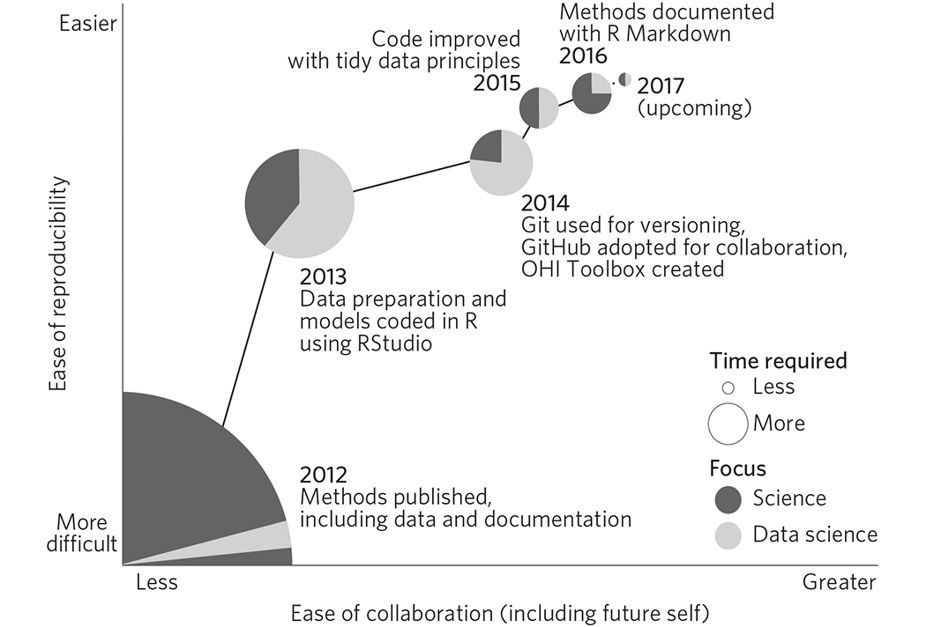
\includegraphics[height=.7\textheight]{figures/Ocean-Health-Index.jpg}
        \caption{Better science in less time, illustrated by the Ocean Health Index project. \cite{Stewart_Lowndes2017-lj}}
        \label{fig:stewart_lowndes}
  \end{figure}
\end{frame}

\begin{comment}

\section{From current practice to better practice}

\begin{frame}{What does this mean? Are we ready?}
  Emerging good practice - and publisher and funder policies - mean:
    \begin{itemize}[label=\textbullet]
        \item Comprehensive, FAIR datasets will be deposited in domain-specific repositories. Data, and especially metadata, quality will be higher.
        \item Data will be captured digitally as early in research as possible, and provenance / version history maintained.
        \item Research approach, processes, and procedures will be documented.
        \item Data processing and analysis will use code (not Excel!) 
        \item Code will be documented and published for reuse.
        \item Further steps taken for analytical reproducibility (use of OSS, version control, automation, containerisation, etc.). 
    \end{itemize}
\end{frame}

\begin{frame}{Challenges and paths forward}
  How do we get from where we are now to where we want to be?
      \begin{itemize}[label=\textbullet]
        \item Understand the evolving expectations of transparent research. 
        \item Pursue proper training
        \item Look past desktop software (Excel, ARCGIS, Filemaker, Access, etc.).
        \item Use emerging research- and domain-specific solutions (even if imperfect).
        \item Overcome `not invented here'; if a solution exists, use it.
        \item Budget for `ground-up' transparency (data and code). Up-front costs will be high but offer longer-term payoffs (in costs, time, and quality).
        \item Implement (and budget for) fundamental good practice in data and code management before other technologies.
        \item Improve research design (prioritise approach over methods) \cite{Muthukrishna2019-kt, Hole1973-cy}
    \end{itemize}
\end{frame}

\end{comment}

\section{`Small data' infrastructure across the data lifecycle}

\begin{frame}{`Small data' research}
 \begin{figure}[H]
    \centering
        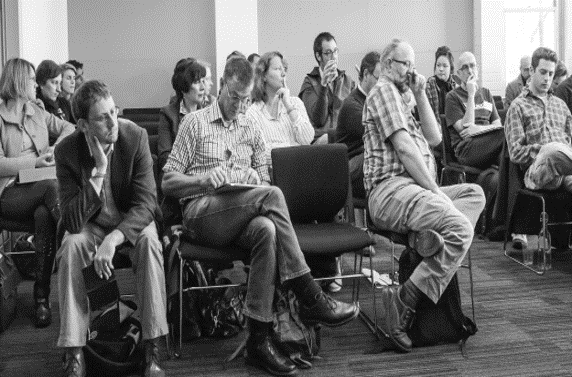
\includegraphics[height=.75\textheight]{figures/Archaeologists-standards.png}
        \caption{Archaeologists contemplate data standards (FAIMS Stocktaking, 2012)}
        \label{fig:figure7}
 \end{figure}
\end{frame}

\begin{frame}{Context: the challenge of `small data'}
    `Long tail' research: most field data is small data \cite{Borgman2015-rh}
    \begin{itemize}[label=\textbullet]
        \item Smaller scale; smaller communities; local control.
        \item Diverse questions, approaches, and methods.
        \item Heterogeneous data; variety of content, structure.
        \item Data and infrastructure emerge from fieldwork. 
        \item Relative lack of standards.
        \item Limited infrastructure and funding.
        \item Challenges associated with big(ger) data from photogrammetry, SfM, video, geophysics, etc., will exacerbate these problems.
    \end{itemize}
\end{frame}

\begin{frame}{The data lifecycle}
 \begin{figure}[H]
    \centering
        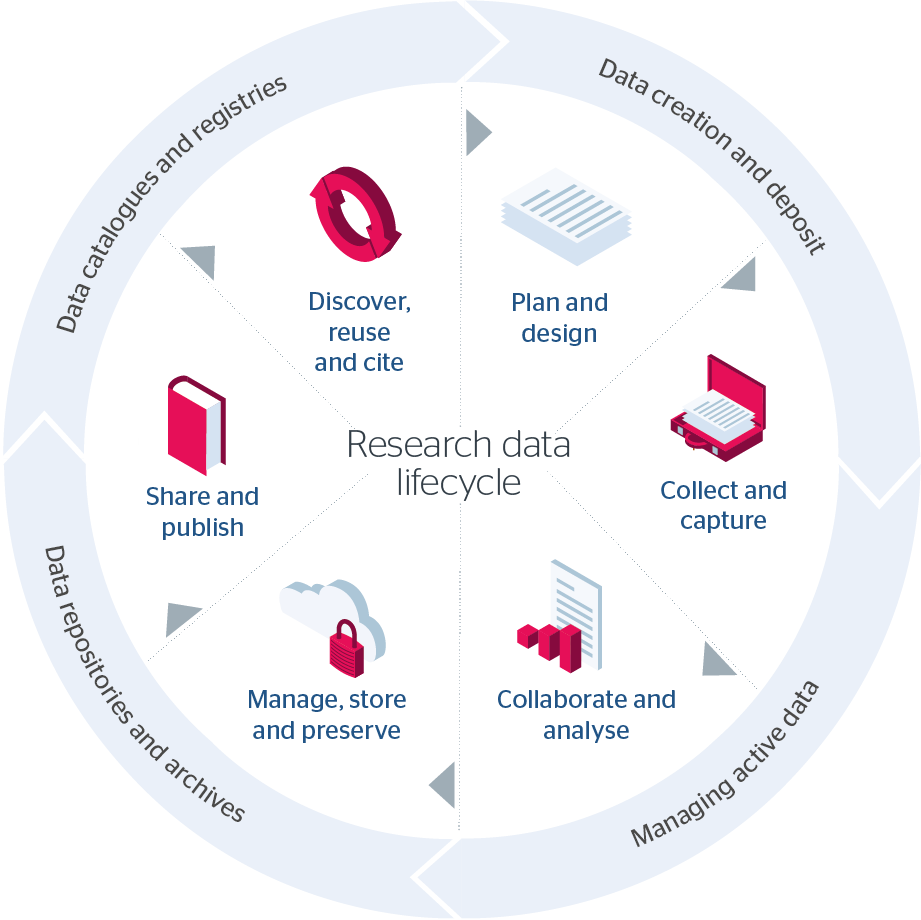
\includegraphics[height=.75\textheight]{figures/research-data-life-diagram.png}
        \caption{\cite{Jisc2018-gx} Image CC-BY-ND}
        \label{fig:figure9}
 \end{figure}
\end{frame}

\begin{frame}{Infrastructure across the data lifecycle}
    Consider the infrastructure needed to manage the three main phases of the data lifecycle
    \begin{itemize}[label=\textbullet]
        \item Publication (most mature): domain-specific repositories.
        \item Processing and analysis (less mature): project-level code \cite{Stewart_Lowndes2017-lj}, then Virtual Labs / Science Gateways, \cite{Alveo2019-tk}.
        \item Capture (least mature): most varied, needs to work offline under difficult conditions. Existing commercial solutions insufficient \cite{Bureau_of_Reclamation2017-xl}.
    \end{itemize}
\end{frame}


% Slides to speak to at WSU 5 June 2019

\section{The FAIMS approach: summary}

\begin{frame}{Research Specific}
 \begin{figure}[H]
    \centering
        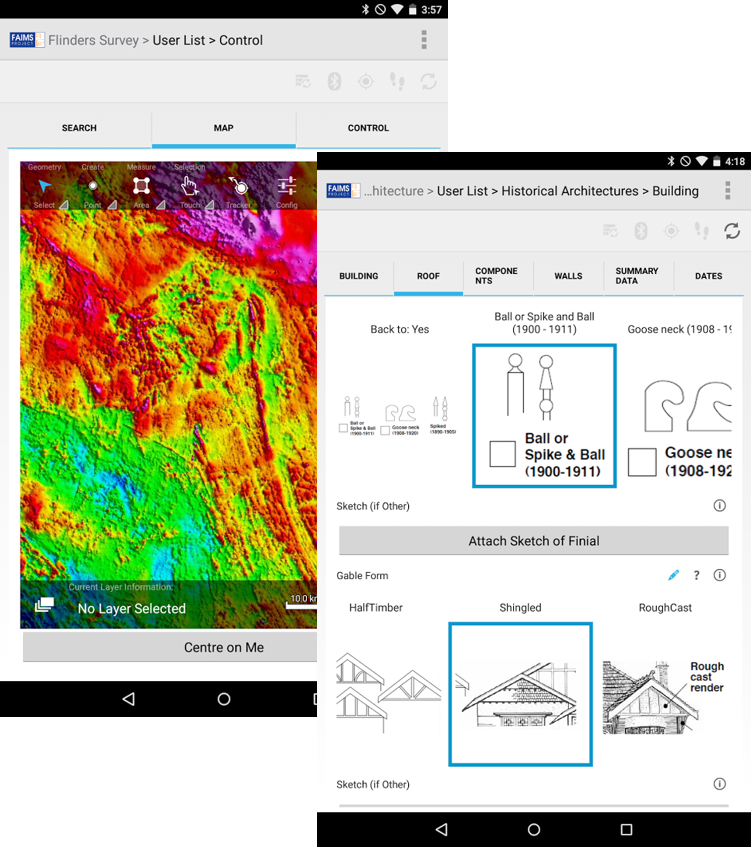
\includegraphics[height=.75\textheight]{figures/FAIMS-screenshots.png}
        \caption{FAIMS Mobile: GIS and `picture dictionaries'}
        \label{fig:FAIMS-mobile-screenshots}
 \end{figure}
\end{frame}


\begin{frame}{Generalised}
 \begin{figure}[H]
    \centering
        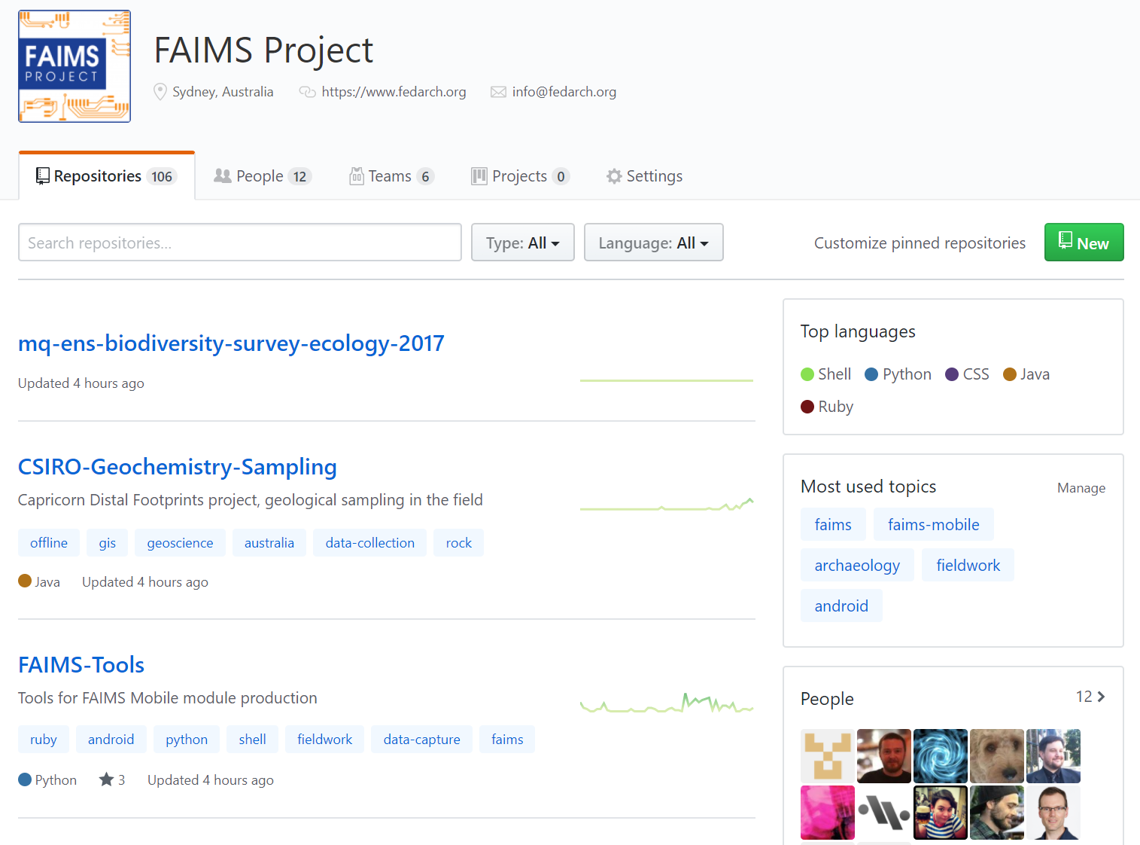
\includegraphics[height=.75\textheight]{figures/FAIMS-generalised.png}
        \caption{FAIMS Mobile customisations on GitHub}
        \label{fig:FAIMS-github}
 \end{figure}
\end{frame}

\begin{frame}{Modular and federated}
 \begin{figure}[H]
    \centering
        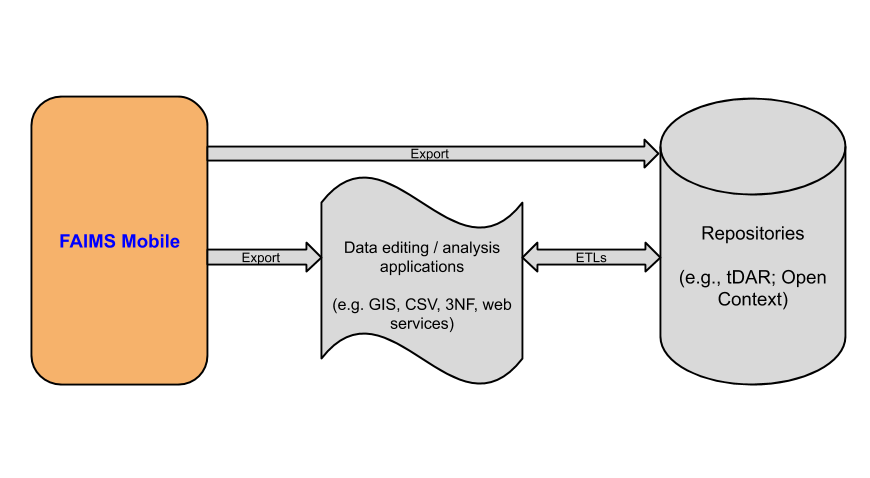
\includegraphics[height=.75\textheight]{figures/FAIMS-federation}
        \caption{FAIMS Mobile federation}
        \label{fig:FAIMS-federation}
 \end{figure}
\end{frame}

\begin{frame}{Open Source}
 \begin{figure}[H]
    \centering
        
\includegraphics[width=.75\textwidth]{figures/GPLv3_Logo.eps}
        \caption{FAIMS Mobile 'core' code is GPLv3; 'module' (customisation) code is also open; everything is on GitHub}
        \label{fig:FAIMS-github-OSS}
 \end{figure}
\end{frame}

\begin{comment}


\begin{frame}{Key research-specific FAIMS Mobile features}
    \begin{itemize}[label=\textbullet]
        \item Fundamentally customisable (interpreter + definition files).
        \item Tightly binds structured, geospatial, multimedia, and free text data.
        \item Works offline.
        \item Automated bi-directional synchronisation using local or online server
        \item Record history: append-only datastore, versioning, rollback.
        \item Mobile GIS.
        \item Connects to internal and external sensors, Bluetooth / USB devices.
        \item Multilingual.
        \item Granular help.
        \item Granular metadata / uncertainty.
        \item Generalised export.
        \item `Hooks’ for data interoperability, Open Linked Data approaches.
    \end{itemize}
\end{frame}

\begin{frame}{Selected FAIMS Testimonials}
    \begin{itemize}[label=\textbullet]
    \item ``The tablet app worked very well in the field and I would be keen to continue using it for subsequent sampling'' -- New Zealand Soil Geochemistry
    \item ``Being able to check in on everyone's work from my computer so easily is... revolutionary. Thank you for building such an amazing tool! …  I look forward to providing more details, but I already feel like I have 100\%{} better control over data quality, even compared to last year'' -- Proyecto Arquelogico de Zana Colonial
    \end{itemize}
\end{frame}

\begin{frame}{Selected FAIMS Testimonials 2}
    \begin{itemize}[label=\textbullet]
    \item ``The app has been such an incredible advantage in terms of workload, data quality, and a number of other data management issues with which archaeologists regularly have to deal. It readily links disparate data types that are otherwise stored separately – such as photographs, tabular logs, and context relationships.'' -- Malawi Early-Middle Stone Age Project
    \item ``I was really impressed with the approach FAIMS project has taken to the challenge of creating field data apps which can be very expensive. Our module was ready for testing after just one briefing.'' -- Streamwatch
    \end{itemize}
\end{frame}

\begin{frame}{Selected FAIMS Testimonials 3}
    \begin{itemize}[label=\textbullet]
\item 
``We’re back from the field and I cannot believe how well everything went. ... [T]he combination of the mobile lab, the sample ID/tracking and FAIMS application enabled us to average 5-6 minutes per sample site (crust, soil, rock and two plants)  in the field and about half that in the lab... Using the old school notepad and GPS approach this would have been 15 mins at best and a whole lot of misplaced photos and details, not to mention the additional hours entering the data in at night. We were able to identify missed sites as we went and completed the soils map (280 sites) and infill (36 sites) and analysis all in the 7 days. '' -- CSIRO Mineral Resources
\end{itemize}
\end{frame}

\begin{frame}{Status and plans for the future}
    \begin{itemize}[label=\textbullet]
        \item FAIMS v2.6 is nearing end of its useful life.
        \item A high-level technical plan for FAIMS v3.0 won a US design prize in 2017 \cite{Bureau_of_Reclamation2017-xl}.
        \item Any future iteration of FAIMS must be sustainable via commercialisation as a (primarily) self-service platform.
        \item The FAIMS team did CSIRO ON Prime in 2016, completing 70+ interviews with clients / potential clients.
        \item We are considering applying for an ARDC Platforms and Services grant, if we can reconcile that with commercialisation.
        \item Challenge: balancing open research / OSS with commercialisation.
    \end{itemize}
\end{frame}

\begin{frame}{Technical improvements}
    \begin{itemize}[label=\textbullet]
        \item Cross-platform support (Android; iOS; desktop)
        \item Self-customisation by the user via a GUI-based web application.
        \item Orchestrated deployment of infrastructure to (e.g.) Amazon Web Services.
        \item Data 'round-trip' to external desktop or online software.
        \item Exposure of data via an API
        \item Improved scalability (application performance; synchronisation performance; server-to-server synchronisation)
        \item Improved user management and security
    \end{itemize}
\end{frame}

\end{comment}

\begin{frame}{FAIMS publications}
Available at: \url{https://paperpile.com/shared/yk95gS}

      \begin{itemize}[label=\textbullet]
      
      
      {\small
      \nocite{Sobotkova2015-lq,Sobotkova2018-al,VanValkenburgh2018-hv,Ballsun-Stanton2018-zd,Sobotkova2016-mx,Ross2015-ph,Ross2013-hi}
        % \item \nocite{Sobotkova2018-al}
        % \item \nocite{Ballsun-Stanton2018-zd}
        % \item \nocite{VanValkenburgh2018-hv}
        % \item \nocite{sobotkova2016-mx}
        % \item \nocite{Ross2015-ph} 
        % \item \nocite{Sobotkova2015-lq}
        % \item \nocite{Ross2013-hi}
\item Ballsun-Stanton, Brian, Shawn A. Ross, Adela Sobotkova, and Penny Crook. 2018. ``FAIMS Mobile: Flexible, Open-Source Software for Field Research.''
\item Ross, Shawn Adrian, Brian Ballsun-Stanton, Adela Sobotkova, and Penny Crook. 2015. ``Building the Bazaar: Enhancing Archaeological Field Recording Through an Open Source Approach.''
\item Ross, Shawn Adrian, Adela Sobotkova, Brian Ballsun-Stanton, and Penny Crook. 2013. ``Creating Eresearch Tools For Archaeologists: The Federated Archaeological Information Management Systems Project.''
\item Sobotkova, Adela. 2018. ``Sociotechnical Obstacles to Archaeological Data Reuse.'' 

}
    \end{itemize}
\end{frame}

\begin{frame}{FAIMS Publications 2}
\begin{itemize}[label=\textbullet]
{\small
    \item Sobotkova, Adela, Brian Ballsun-Stanton, Shawn Ross, and Penny Crook. 2015. ``Arbitrary Offline Data Capture on All of Your Androids: The FAIMS Mobile Platform.''
\item Sobotkova, Adela, Shawn A. Ross, Brian Ballsun-Stanton, Andrew Fairbairn, Jessica Thompson, and Parker VanValkenburgh. 2016. ``Measure Twice, Cut Once: Cooperative Deployment of a Generalized, Archaeology-Specific Field Data Collection System.'' 
\item VanValkenburgh, Parker, Luiza O. G. Silva, Chiara Repetti-Ludlow, Jake Gardner, Jackson Crook, and Brian Ballsun-Stanton. 2018. ``Mobilization as Mediation: Implementing a Tablet-Based Recording System for Ceramic Classification.''} 
\end{itemize}
    
\end{frame}
\begin{frame}{Thank you!}

%This presentation is available at:
%\texttt{https://osf.io/v5jp7/}

PDF and source code for this presentation is available at: 
\texttt{https://github.com/saross/Open-HASS/releases/tag/v1.0}

FAIMS Project software and documentation can be found at:
\texttt{https://github.com/faims}.

This work is licensed under a Creative Commons Attribution 4.0 International License.

\end{frame}

% In-depth information for reference
\section{The FAIMS approach: in-depth}

\begin{frame}{Introduction to the FAIMS Project}
    \begin{itemize}[label=\textbullet]
        \item The Field Acquired Information Management Systems (FAIMS) Project began in 2012 as a national Australian information infrastructure project in archaeology.
        \item Developed FAIMS Mobile for field data capture \cite{Ballsun-Stanton2018-zd}.
        \item Use expanded beyond archaeology to geoscience, ecology, ethnography, linguistics, oral history.
        \item Has been customised for over 50 workflows at more than 30 projects. 
        \item Data and workflow modelling for customisations provided deep insights into field data capture and the infrastructure needed to support it.
    \end{itemize}
\end{frame}

\begin{frame}{FAIMS Mobile software}
 \begin{figure}[H]
    \centering
        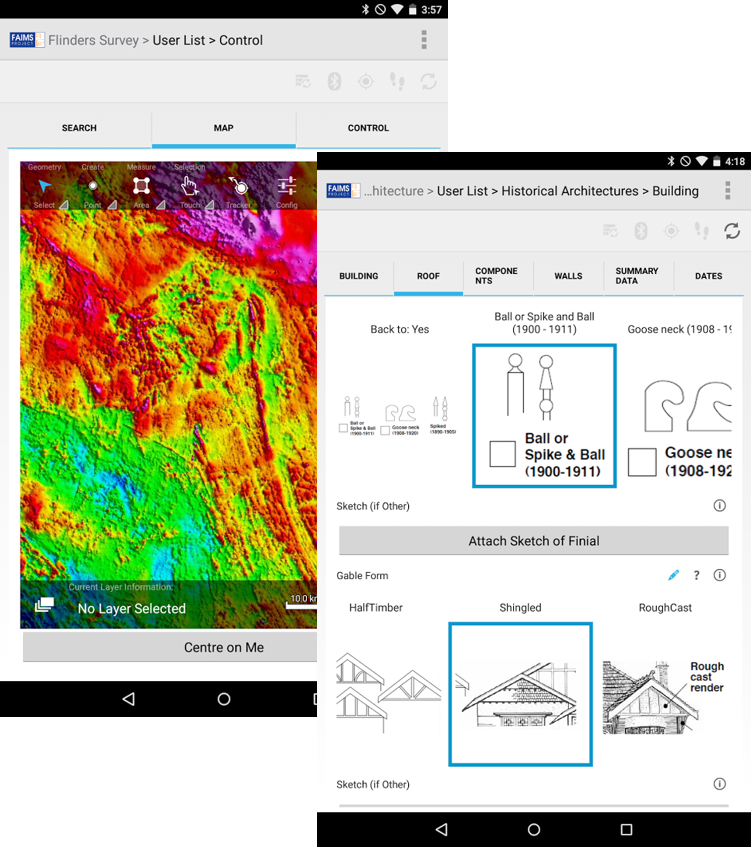
\includegraphics[height=.75\textheight]{figures/FAIMS-screenshots.png}
        \caption{FAIMS Mobile: GIS and `picture dictionaries'}
        \label{fig:figure10}
 \end{figure}
\end{frame}

\begin{frame}{Field data capture infrastructure: a manifesto}
    \begin{itemize}[label=\textbullet]
        \item Our domains deserve research-specific software.
        \item Diverse practices and limited resources require generalised software.
        \item Do one thing well with modular and federated software (but slice the pie thoughtfully).
        \item Open-source software supports open research and has other advantages (but is difficult to sustain). 
        \item Scope requirements carefully.
        \item Invest in outreach and engagement.
    \end{itemize}
\end{frame}

\begin{frame}{Research specific}
    Field research needs (and deserves) research-specific software, contra \cite{Roosevelt2015-kd}.
      \begin{itemize}[label=\textbullet]
        \item Most commercial / mass-market software does not meet research needs.
        \item Risk of lock-in, unwelcome changes to features or business models, and product discontinuation.
    \end{itemize}
    Compare ecology: TERN, ALA, Biocollect, and associated research clouds \cite{Tern2019-sp, Ala2019-by, Ala2019-cb}.
\end{frame}

\begin{frame}{Generalised (not generic or bespoke)}
  Commercial software doesn't meet our needs, and bespoke development is too expensive and usually unsustainable.
      \begin{itemize}[label=\textbullet]
        \item Generalised software can be deeply customised to accommodate our diverse data types, data models, workflows, etc.
        \item The code used to customise it describes the data model and workflow.
        \item Customisations can be published and re-deployed trivially.
        \item Can deliver research-grade software affordably.  
    \end{itemize}
    FAIMS Mobile cost perhaps 3x a single bespoke application, but has been customised 50x. Customisation cost is 1/10th bespoke, and still <1/2 even if `core' platform development costs are amortised across projects.
\end{frame}

\begin{frame}{Generalised: customise using code}
 \begin{figure}[H]
    \centering
        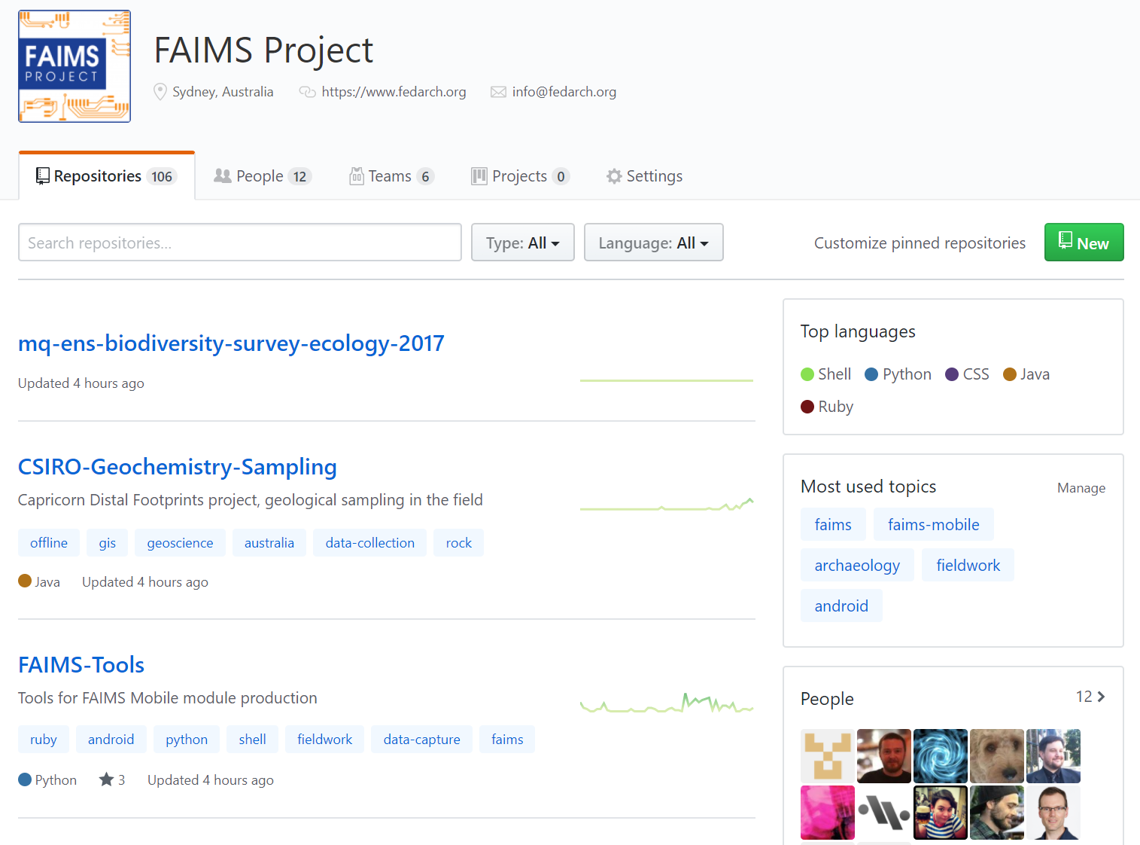
\includegraphics[height=.75\textheight]{figures/FAIMS-generalised.png}
        \caption{FAIMS Mobile customisations (XML files, mostly) on GitHub}
        \label{fig:figure11}
 \end{figure}
\end{frame}

\begin{frame}{Modular and federated}
  Do one thing well.
      \begin{itemize}[label=\textbullet]
        \item Identify other infrastructure in the domain and interoperate with it (via ETLs or APIs).
        \item It is better to divide by data-lifecycle phase rather than data type, since (1) our data is so integrated and (2) field data capture poses unique challenges.
    \end{itemize}
\end{frame}

\begin{frame}{Modularise by data lifecycle phase}
 \begin{figure}[H]
    \centering
        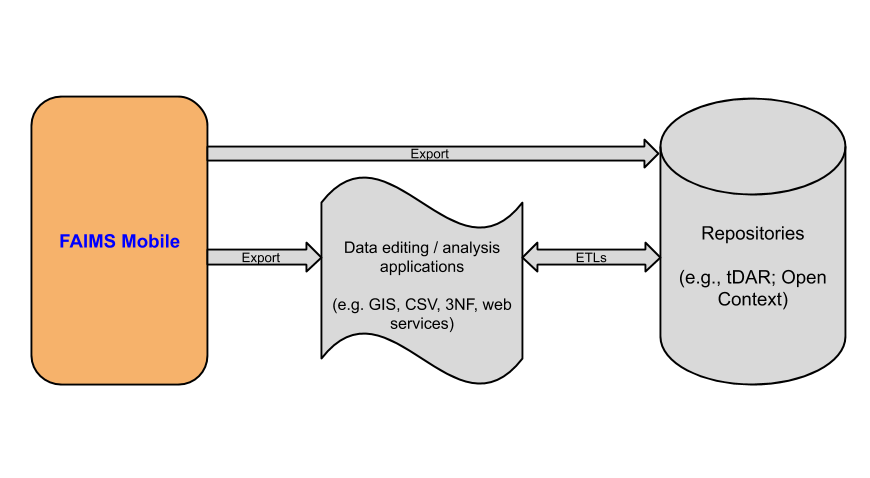
\includegraphics[height=.75\textheight]{figures/FAIMS-federation.png}
        \caption{FAIMS Mobile federation strategy}
        \label{fig:figure13}
 \end{figure}
\end{frame}

\begin{frame}{Open source?}
  Open source has advantages but is difficult to sustain.
      \begin{itemize}[label=\textbullet]
        \item Emerging open research principles strongly prefer OSS as opposed to proprietary ‘black boxes’.
        \item Transparency and reusability (esp. customisation code).
        \item Ability to hand off from one organisation to another (esp. `core' platform code).
        \item Ability to fork code prevents lock-in and mitigates unwelcome decisions by software developers.
        \item BUT OSS business models are hard to scale and rely on occasional injections of grant or institutional funding.
    \end{itemize}
\end{frame}

\begin{frame}{Scope carefully}
  Talk to a wide range of potential users, seeking facts not opinions.
      \begin{itemize}[label=\textbullet]
        \item Don’t ask researchers what they think, ask them what they have done - what software they have adopted and why, and what problems they have expended resources to solve. 
        \item ‘Lean startup’ methodology very useful, based around  testing of ideas through interviews with potential users \cite{Strategyzer_AG2019-uu}.
        \item In our case, we over-invested in mobile GIS and under-invested in usability (especially a GUI for customisation).
    \end{itemize}
\end{frame}

\begin{frame}{Spend on outreach and engagement}
  If you build it they will not come; people can't use technologies they don't know about.
      \begin{itemize}[label=\textbullet]
        \item As per industry standards, dedicate at least 30\% of any information infrastructure budget to outreach and engagement (sales and marketing). 
        \item Typical academic outreach (journal articles, conference presentations, workshops, even booths at major conferences) are not enough.
    \end{itemize}
\end{frame}

% \bibliographystyle{apalike}

% Adding the option 'allowframebreaks' allows the contents of the slide to be expanded in more than one slide.
% The "1" comes from the outer theme"

\section{References}

\begin{multicols}{2}[]
\bibliography{references}
\bibliographystyle{apalike}
\end{multicols}


% \begin{frame}[allowframebreaks]{References}
  
%   \bibliography{references}
%   \bibliographystyle{apalike}
% \end{frame}

\end{document}